% AnchorMTM with updated correspondence and Storms teaser, 2026-11-02.
% Build: tectonic -X compile --keep-logs method_anchor_figures_updated_en.tex
% Unchanged companion: method_anchor_single_parameter_supplement.tex/.pdf.
% Changes: ANCHORMTM_SINGLE_PARAMETER_VALIDATION.md.
\documentclass[review]{vgtc}
\usepackage[T1]{fontenc}
\usepackage{mathptmx}
\usepackage{cite}
\usepackage{amsmath,amssymb,amsthm}
\usepackage{placeins}
\usepackage{float,stfloats,needspace}
\usepackage{booktabs,multirow,colortbl}
\makeatletter
\setlength{\@dblfptop}{0pt}
\setlength{\@dblfpsep}{12pt}
\setlength{\@dblfpbot}{0pt plus 1fil}
\makeatother
\usepackage[ruled,vlined]{algorithm2e}
\SetKwInput{KwData}{Data}
\SetKwInput{KwResult}{Result}
\SetKwProg{Fn}{Function}{:}{}
\SetKw{KwReturn}{return}
\SetKw{KwBreak}{break}
\SetKwFunction{Construct}{ConstructTemporalMap}
\SetKwFunction{Refine}{RefineOrder}
\SetKwFunction{Barriers}{OptimalBarriers}
\SetAlFnt{\small}
\SetAlCapFnt{\small\bfseries}
\SetAlCapNameFnt{\small\bfseries}
\SetAlCapSkip{3pt}
\DontPrintSemicolon
\setcounter{secnumdepth}{3}
\newtheorem{theorem}{Theorem}
\newtheorem{lemma}{Lemma}
\newtheorem{proposition}{Proposition}
\newcommand{\dtop}{d_{\mathrm{top}}}
\newcommand{\lca}{\operatorname{lca}}
\newcommand{\nroe}{\mathrm{NROE}}
\newcommand{\pos}[1]{\left[#1\right]^+}
\title{AnchorMTM: Spatially Anchored Merge Tree Maps\\for Time-Varying Scalar Fields}
\author{Anonymous Authors}
\onlineid{0}
\vgtccategory{Research}
\vgtcinsertpkg
\hypersetup{pdftitle={AnchorMTM: Spatially Anchored Merge Tree Maps for Time-Varying Scalar Fields},pdfauthor={Anonymous Authors}}
\abstract{Temporal merge tree maps summarize the hierarchy of a time-varying scalar field, but their display coordinate does not provide a fixed spatial reference. Anchoring this coordinate reveals a structural conflict: exact topology requires contiguous subtree blocks, whereas projected feature positions can interleave. We quantify the resulting positional cost through three layout-independent bounds for exact point orders, finite-width interval layouts and bounded merge-level error. AnchorMTM uses these bounds to guide leaf-order selection and capped anchor placement, then reconstructs scalar profiles under a controlled merge budget. Controlled four-leaf experiments compare the bounds with exhaustive ordering and independent linear programs. Existing results on five planar and two volumetric sequences then connect unavoidable displacement, absolute positioning and the effect of relaxation. The per-frame evidence shows that a budget resolves a difficult tail of Storms frames and shifts most frames in the default volume configurations. The resulting maps make feature positions readable against one shared spatial direction while exposing the hierarchical cost of that coordinate.}
\keywords{Time-varying scalar fields, merge tree maps, spatial anchoring, topology preservation, constrained layout.}
\teaser{
\centering
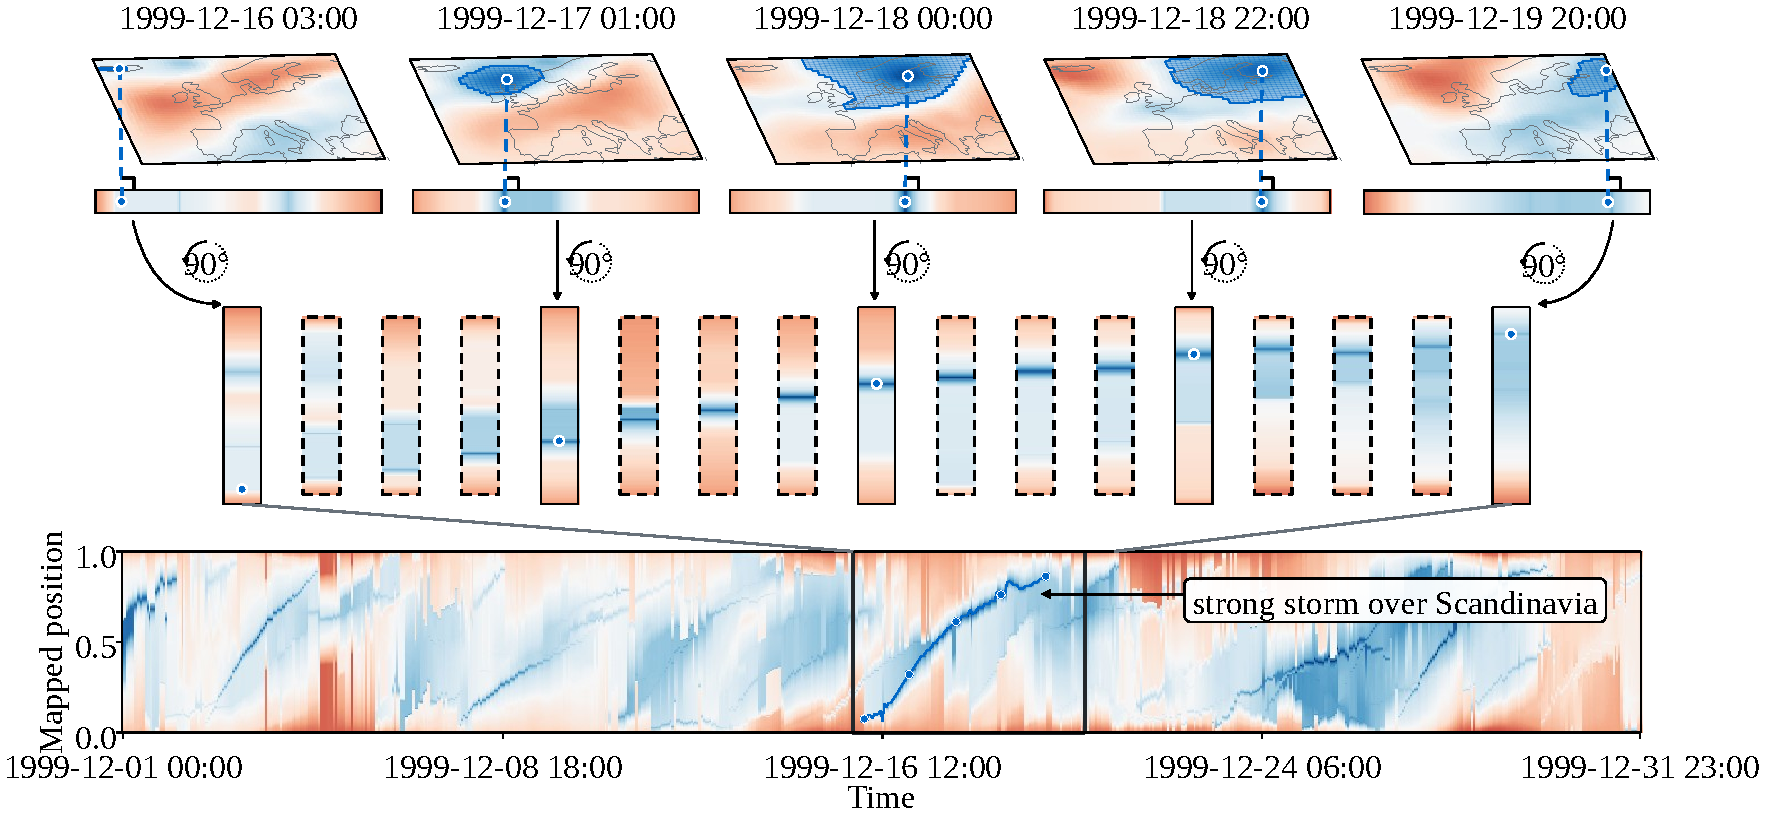
\includegraphics[width=\linewidth]{figures/anchor_storms_overview.pdf}
\par
\refstepcounter{figure}\label{fig:storms_overview}
{\captionfonts\raggedright\noindent\figurename~\thefigure: Storms temporal overview ($\varepsilon=5\%$), using the case-study preprocessing. Spatial snapshots and profiles identify one matched extremum; blue outlines show leaf-arc supports. Rotated profiles and dashed intermediate samples connect to its trajectory in the full 744-frame map.\par}

}
\linespread{1.0}
\setlength{\textfloatsep}{7pt}
\setlength{\floatsep}{6pt}
\setlength{\dbltextfloatsep}{7pt}
\setcounter{dbltopnumber}{2}
\renewcommand{\dbltopfraction}{0.9}
\renewcommand{\dblfloatpagefraction}{0.7}
\renewcommand{\floatpagefraction}{0.7}
\setcounter{totalnumber}{6}
\setcounter{topnumber}{3}
\setcounter{bottomnumber}{3}
\renewcommand{\textfraction}{0.07}

\newcommand{\paperfigure}[4][\textwidth]{\centering\includegraphics[width=#1]{#2}\caption{#4}\label{#3}}


\begin{document}
\firstsection{Introduction}
\maketitle
\raggedbottom
\setlength{\emergencystretch}{1.5em}
Time-varying scalar fields describe phenomena whose structure and location evolve together: storms move, pollution peaks develop, and vortices form and shed. Analysis therefore requires three kinds of information---feature identity and hierarchy, spatial location, and temporal change. Animation retains the field at each instant; static overviews support comparison across distant times~\cite{Tversky:2002:Animation,Robertson:2008:Animation,Bach:2017:STC}. When one display axis represents time, the meaning of the remaining coordinate determines which spatial questions the overview can answer. Figure~\ref{fig:storms_overview} connects these questions through source supports, profiles and feature trajectories.

Temporal Merge Tree Maps (TMTM) address hierarchy and temporal comparison by converting each frame into a one-dimensional scalar profile, with extrema at minima and merges at intervening barriers, and assembling these profiles along time~\cite{Koepp:2023:TMTM}. Spatiotemporal Merge Tree Maps (ST-MTM) extend this foundation with relative spatial geometry and temporal position constraints~\cite{STMTM:2026}. These objectives organize the features coherently, but they do not assign the display axis a fixed physical direction and origin. Consequently, a position cannot directly be read as longitude or distance along a flow, and a trajectory does not by itself express motion along that coordinate.

A spatial reference encounters a structural obstruction. An exact profile keeps every strict subtree contiguous, but projected sibling subtrees can interleave. If leaves $A,B$ belong to one subtree and $C,D$ to another, the reference order $A,C,D,B$ splits the first block. Some features must leave their targets, or some displayed merge levels must change. Finite feature widths add packing costs. The resulting displacement has two causes: a part imposed by the hierarchy and a part introduced by the layout.

The central question is therefore the positional cost of keeping the tree: how much displacement is unavoidable, and how much is introduced by a particular order or placement? We answer progressively for exact point orders, finite-width interval layouts and bounded merge-level error. Recursive midpoint ordering attains the point bound; the interval bounds certify unavoidable cost without asserting that every such certificate is attainable. Because the bounds depend on the tree, reference and widths, they separate structural restrictions from the objectives used to draw a map.

AnchorMTM turns this analysis into a temporal map with one fixed spatial reference. It prepares the trees and feature correspondences, searches orders within a merge budget, optimizes anchors under a displacement cap, and reconstructs the scalar profiles. The evidence follows the same chain: establish the bounds on controlled trees and existing sequences, evaluate absolute positioning, then examine which conflicts a budget releases and how those changes appear in the maps.

Our contributions are:
\begin{itemize}\setlength{\itemsep}{1pt}\setlength{\parsep}{0pt}
\item Three layout-independent position bounds for exact topology, finite widths and bounded merge error.
\item A construction that couples fixed spatial targets with budgeted ordering and capped temporal placement.
\item Controlled-tree validation and planar/volumetric evidence connecting reference displacement, merge budgets and feature trajectories.
\end{itemize}

\section{Related Work}\label{sec:related}
\subsection{Domain-, Feature-, and Topology-Based Summaries}
Static views and animation distribute temporal comparison across space and time~\cite{Tversky:2002:Animation,Robertson:2008:Animation}; generalized space--time cubes describe transformations between these organizations~\cite{Bach:2017:STC}. Hovm\"oller diagrams retain a physical coordinate while aggregating the remaining dimensions~\cite{Hovmoller:1949}. Geographic orderings and space-filling curves traverse the spatial domain~\cite{Guo:2006:SpatialOrder,Dafner:2000:CSFC}, with extensions for volume comparison and scalar-aware traversal~\cite{Weissenboeck:2019:DVL,Zhou:2021:DSF}. Their coordinate records traversal rank, while averaging can merge nearby extrema.

Feature-based approaches organize selected entities and their motion, as in one-dimensional projections and MotionRugs~\cite{Franke:2021:1DP,Buchmueller:2019:MR}. Their emphasis differs from traversing every domain sample. Embeddings more generally balance original-domain relationships against display organization~\cite{Nonato:2019:MP}. Figure~\ref{fig:related-work-mapping} makes the distinction explicit: domain-based traversal retains samples, feature-based summaries select structures of interest, and topology-based profiles retain hierarchical relations. AnchorMTM builds on the last representation and assigns its extrema targets in a fixed physical projection.

\begin{figure}[!tb]
\centering
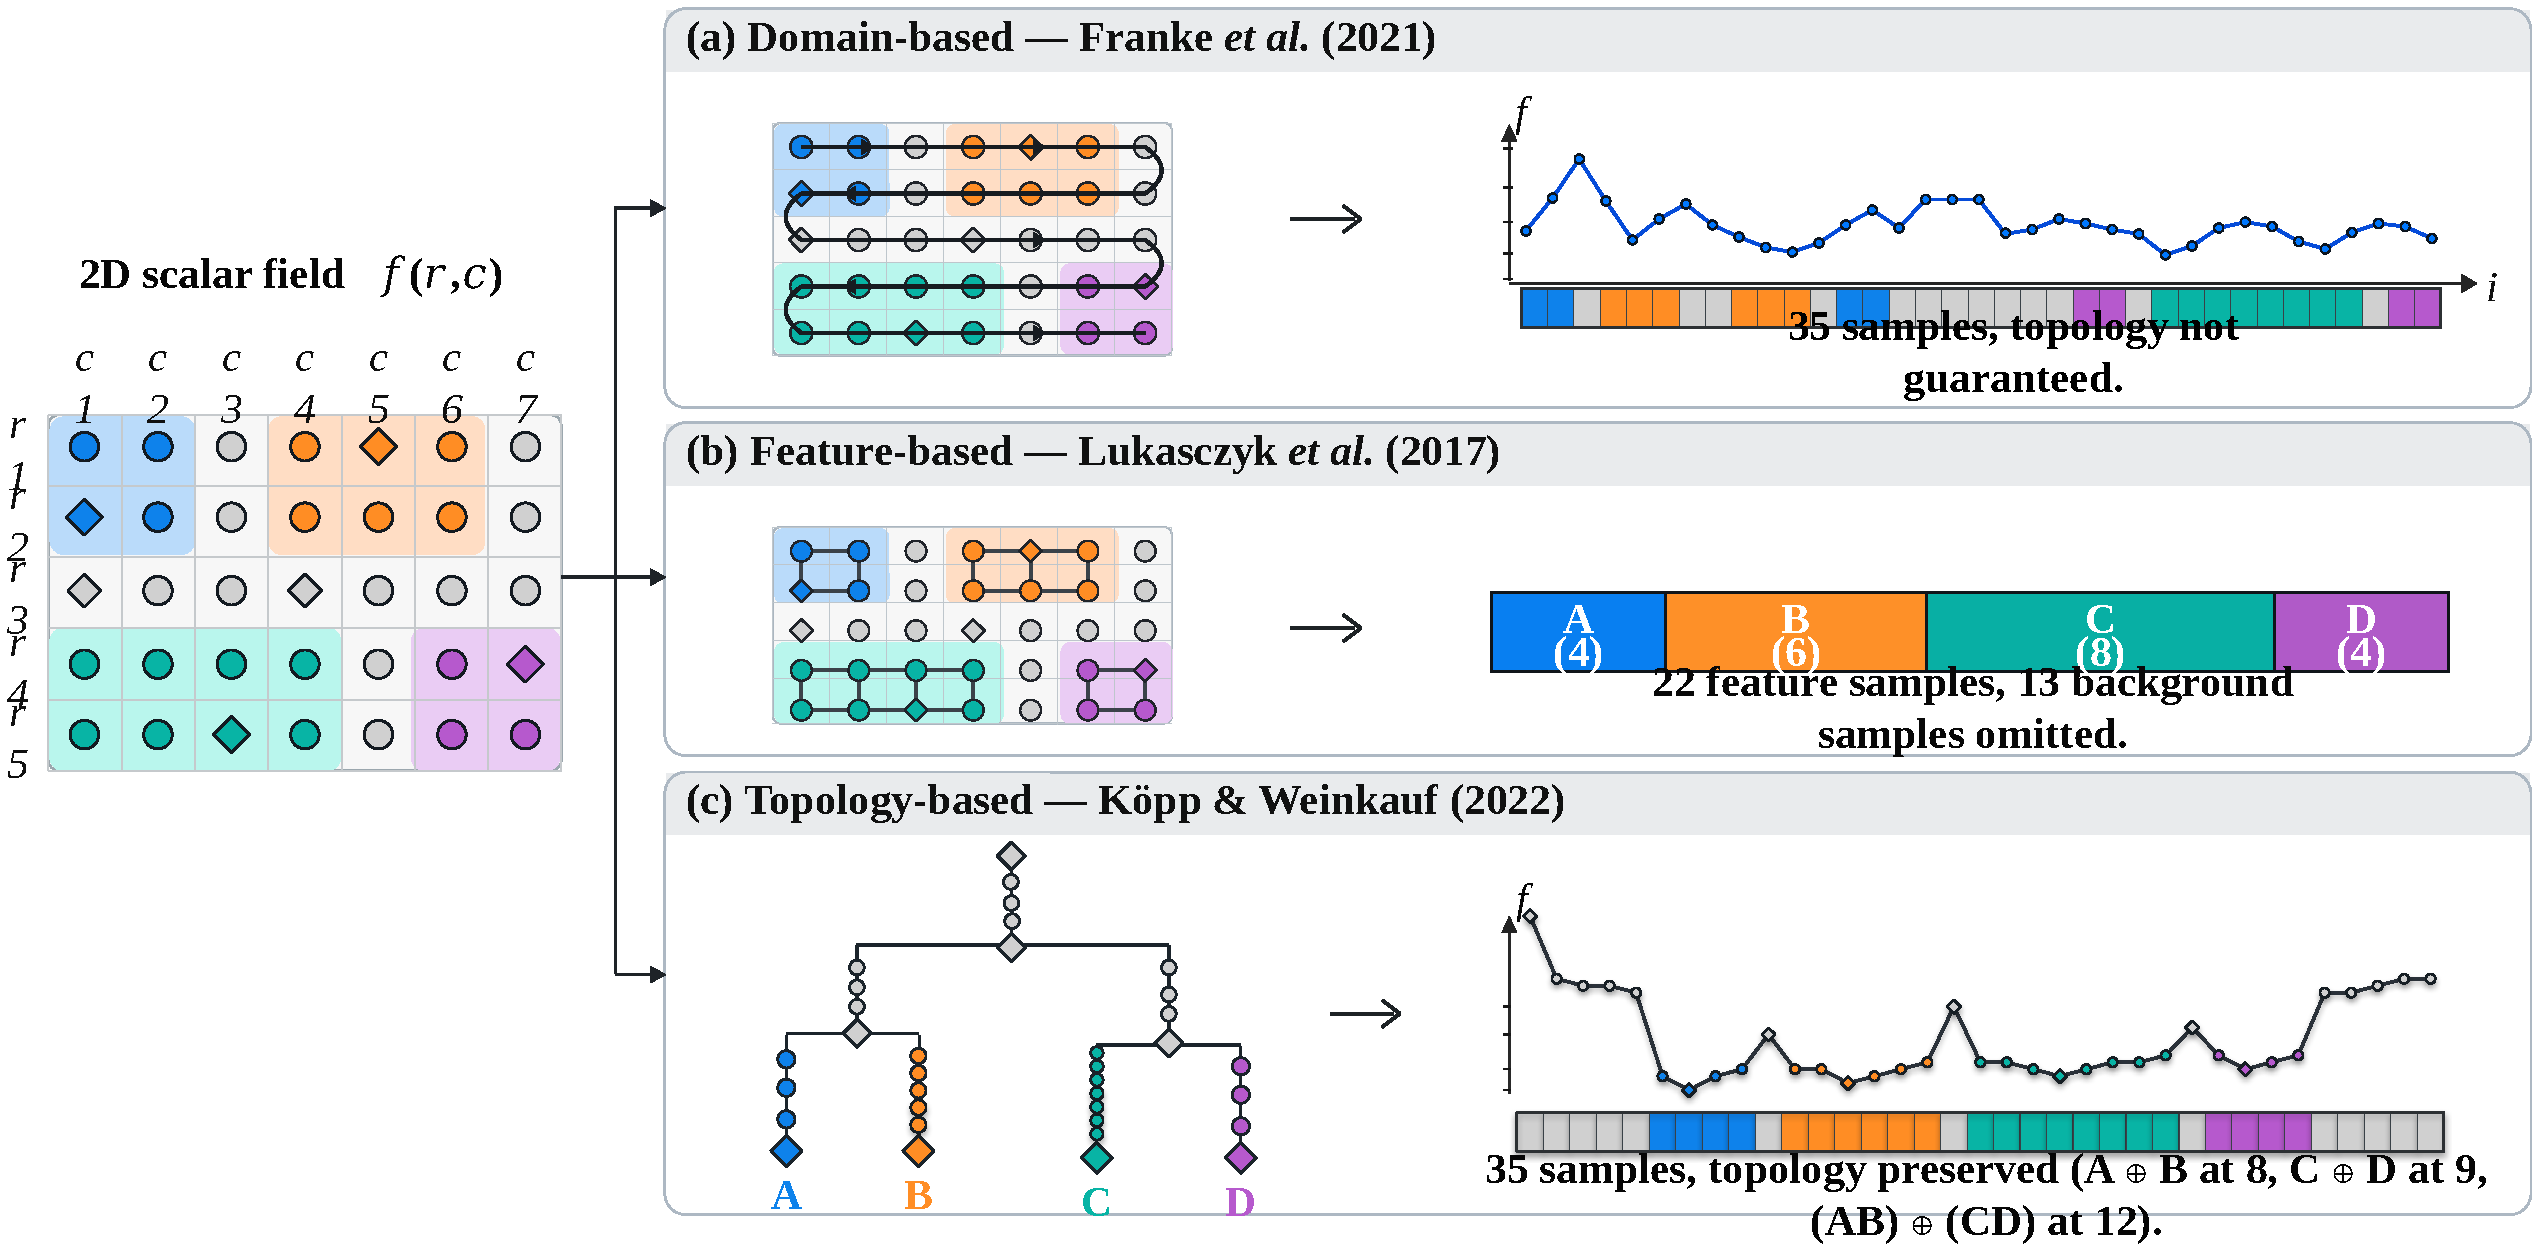
\includegraphics[width=\columnwidth]{figures/anchor_related_work_mapping.pdf}
\caption{Mapping strategies on a common 35-sample field: domain traversal; a 22-sample feature summary; and a topology-based profile retaining the complete illustrated hierarchy.}
\label{fig:related-work-mapping}
\end{figure}
\subsection{Topological Profiles and Constrained Layouts}
Topology-based representations organize scalar structures through connectivity~\cite{Heine:2016:Survey}. Landscapes and profiles turn the hierarchy into geometry~\cite{Weber:2007:TL,Oesterling:2013:TLP}, with extensions for spatial geometry and temporal coherence~\cite{Beketayev:2012:GPTL,Herick:2020:TCTL}. TMTM aligns these profiles through time~\cite{Koepp:2023:TMTM}; ST-MTM incorporates spatial-distance fitting and temporal constraints~\cite{STMTM:2026}. AnchorMTM retains that scalar-profile foundation. Its additional requirement is that one display coordinate refer to the same physical direction, origin and scale throughout the sequence.

Optimal leaf ordering minimizes adjacent dissimilarity subject to a hierarchy~\cite{BarJoseph:2001:OLO}; target-order reordering studies related compatible permutations~\cite{Bulteau:2022:RT}. Separation-constrained layouts manage overlap and displacement~\cite{Dwyer:2006:IPSEP,Li:2019:SOI}. Our bounds state the displacement that these ordering and packing constraints force relative to fixed targets. Merge-tree comparison depends on feature labels and correspondences~\cite{Yan:2021:Survey}; labelled cophenetic/interleaving representations support our fixed-identity merge-error measure~\cite{Munch:2019:LINF,Gasparovic:2024:IID}. Ordered merge trees connect scalar curves with interleaving distances~\cite{Beurskens:2025:OMT}, and minimax ultrametric fitting provides a related setting for correcting merge levels~\cite{Farach:1995:RM}.

\section{Problem Formulation}\label{sec:formulation}\label{sec:background}
\subsection{Merge Trees, Profiles, and Feature Identity}
For a sampled field $f_t$, the merge tree $T_t$ records sublevel components created at minima and joined at saddles; negating the field handles maxima~\cite{Tierny:2018:TTK}. Extraction and persistence simplification precede layout. A leaf $i$ has extremum location $p_i^t$ and support $S_i^t$, comprising the samples on its leaf arc. Augmented internal arcs retain samples for filling the profile. Write $h_t(v)$ for a node's scalar level and $\mathcal{D}_t(v)$ for its descendant leaves. The fixed-label merge matrix is
\begin{equation}\label{eq:merge}
V_{ij}^t=h_t(\lca(i,j)),\quad i\ne j;\qquad V_{ii}^t=f_t(p_i^t).
\end{equation}
Equal-level merges form one multifurcation. A one-dimensional profile $\psi_t$ places the extrema in leaf order $\pi_t$; the largest profile value between anchors $i,j$ gives their displayed merge level $V_{ij}^{\psi_t}$. Exact topology requires each strict subtree to form one contiguous block.

On a fixed grid, one-to-one Hungarian matching maximizes $|S_i^{t-1}\cap S_j^t|$ and discards zero-overlap pairs~\cite{STMTM:2026}. A matched leaf inherits its track identity; $\mu_t(i)$ denotes its predecessor. These links supply the temporal targets and motion samples below. The support is the leaf arc rather than the full component: internal arcs keep their own samples for reconstruction. Matching maximizes intersection counts, so a continuation is an assigned computational correspondence; unmatched leaves create or end tracks. A birth therefore contributes a current reference target but no predecessor target. The same matching is reused for every tested budget, keeping the temporal information fixed while the order constraints change.

\begin{figure}[!tb]
\centering
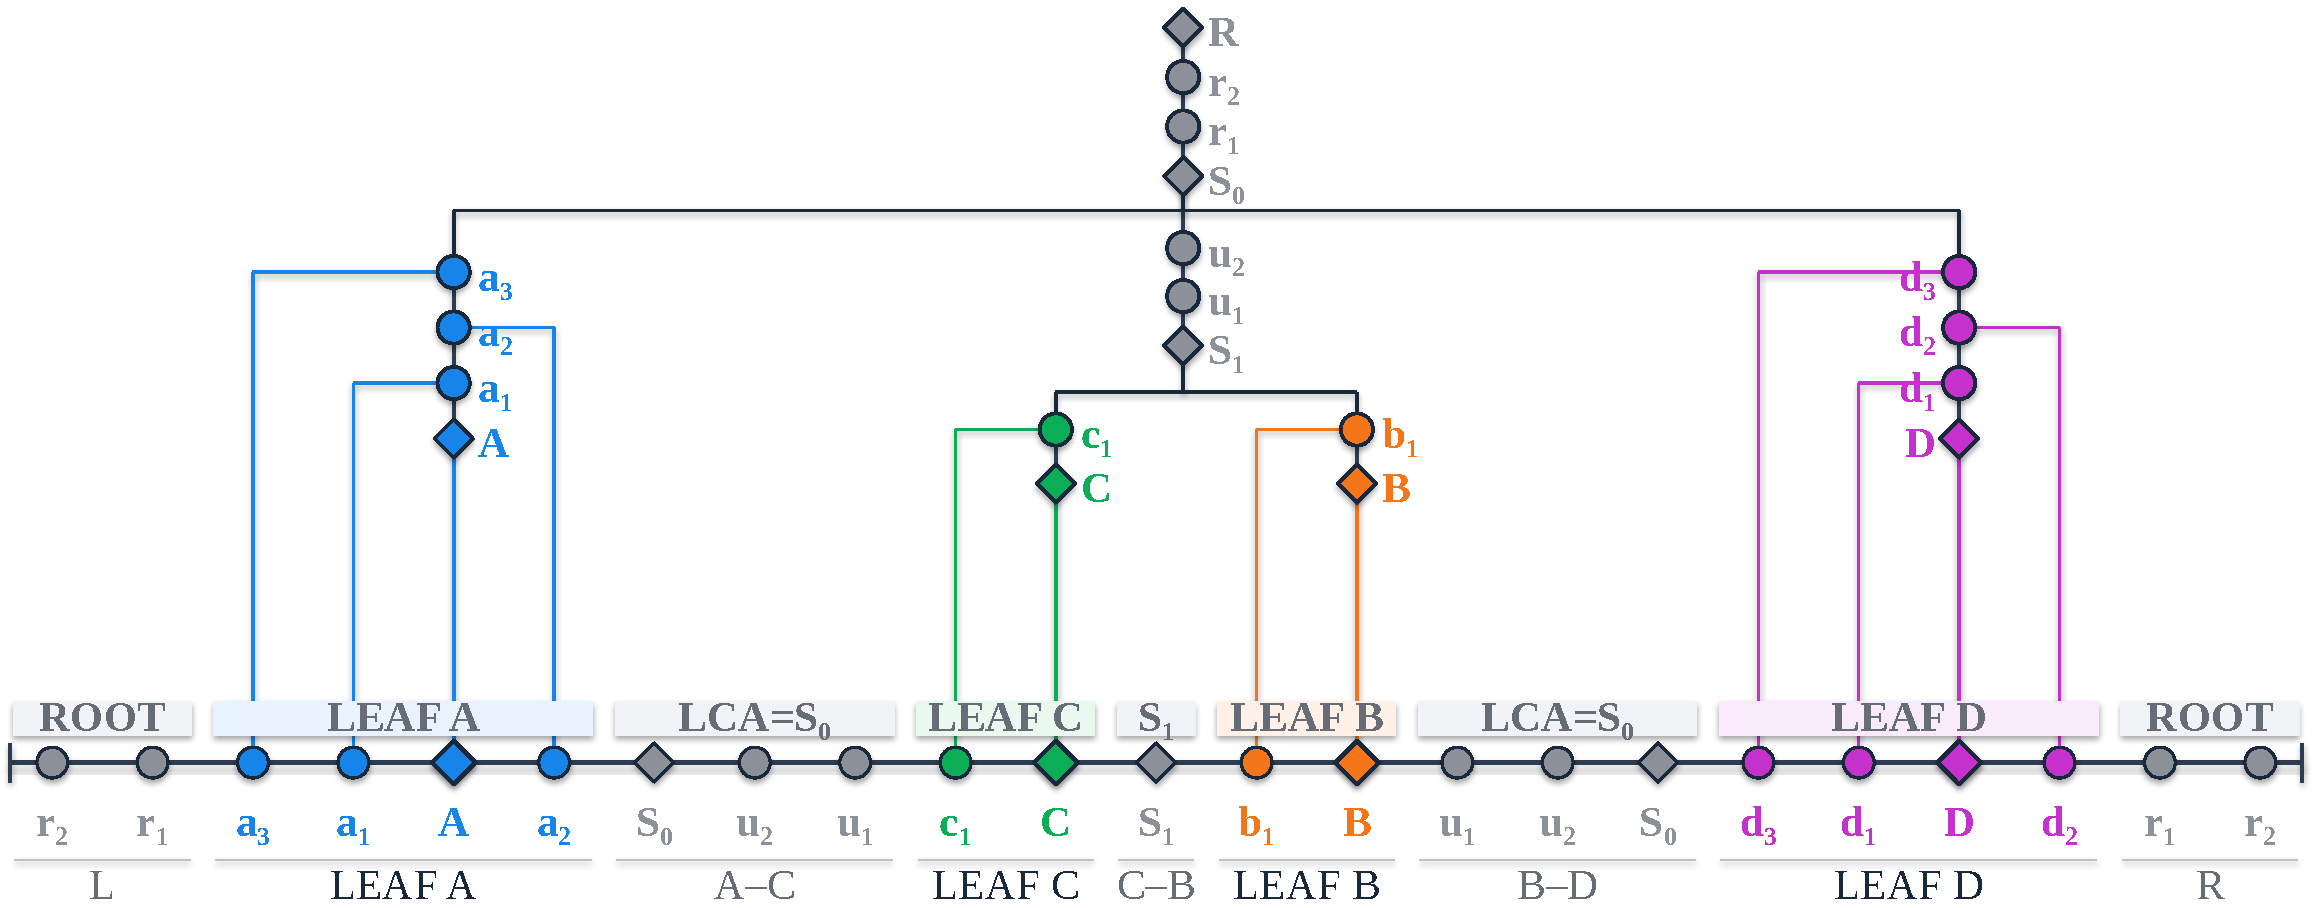
\includegraphics[width=\columnwidth]{figures/anchor_node_mapping.pdf}
\caption{An augmented merge tree and its profile retain the identities of extrema and regular arc samples. Their ordering makes every strict subtree contiguous.}
\label{fig:node-mapping}
\end{figure}
\subsection{Fixed Spatial Reference}\label{sec:reference-model}
\begin{figure}[!tb]
\centering
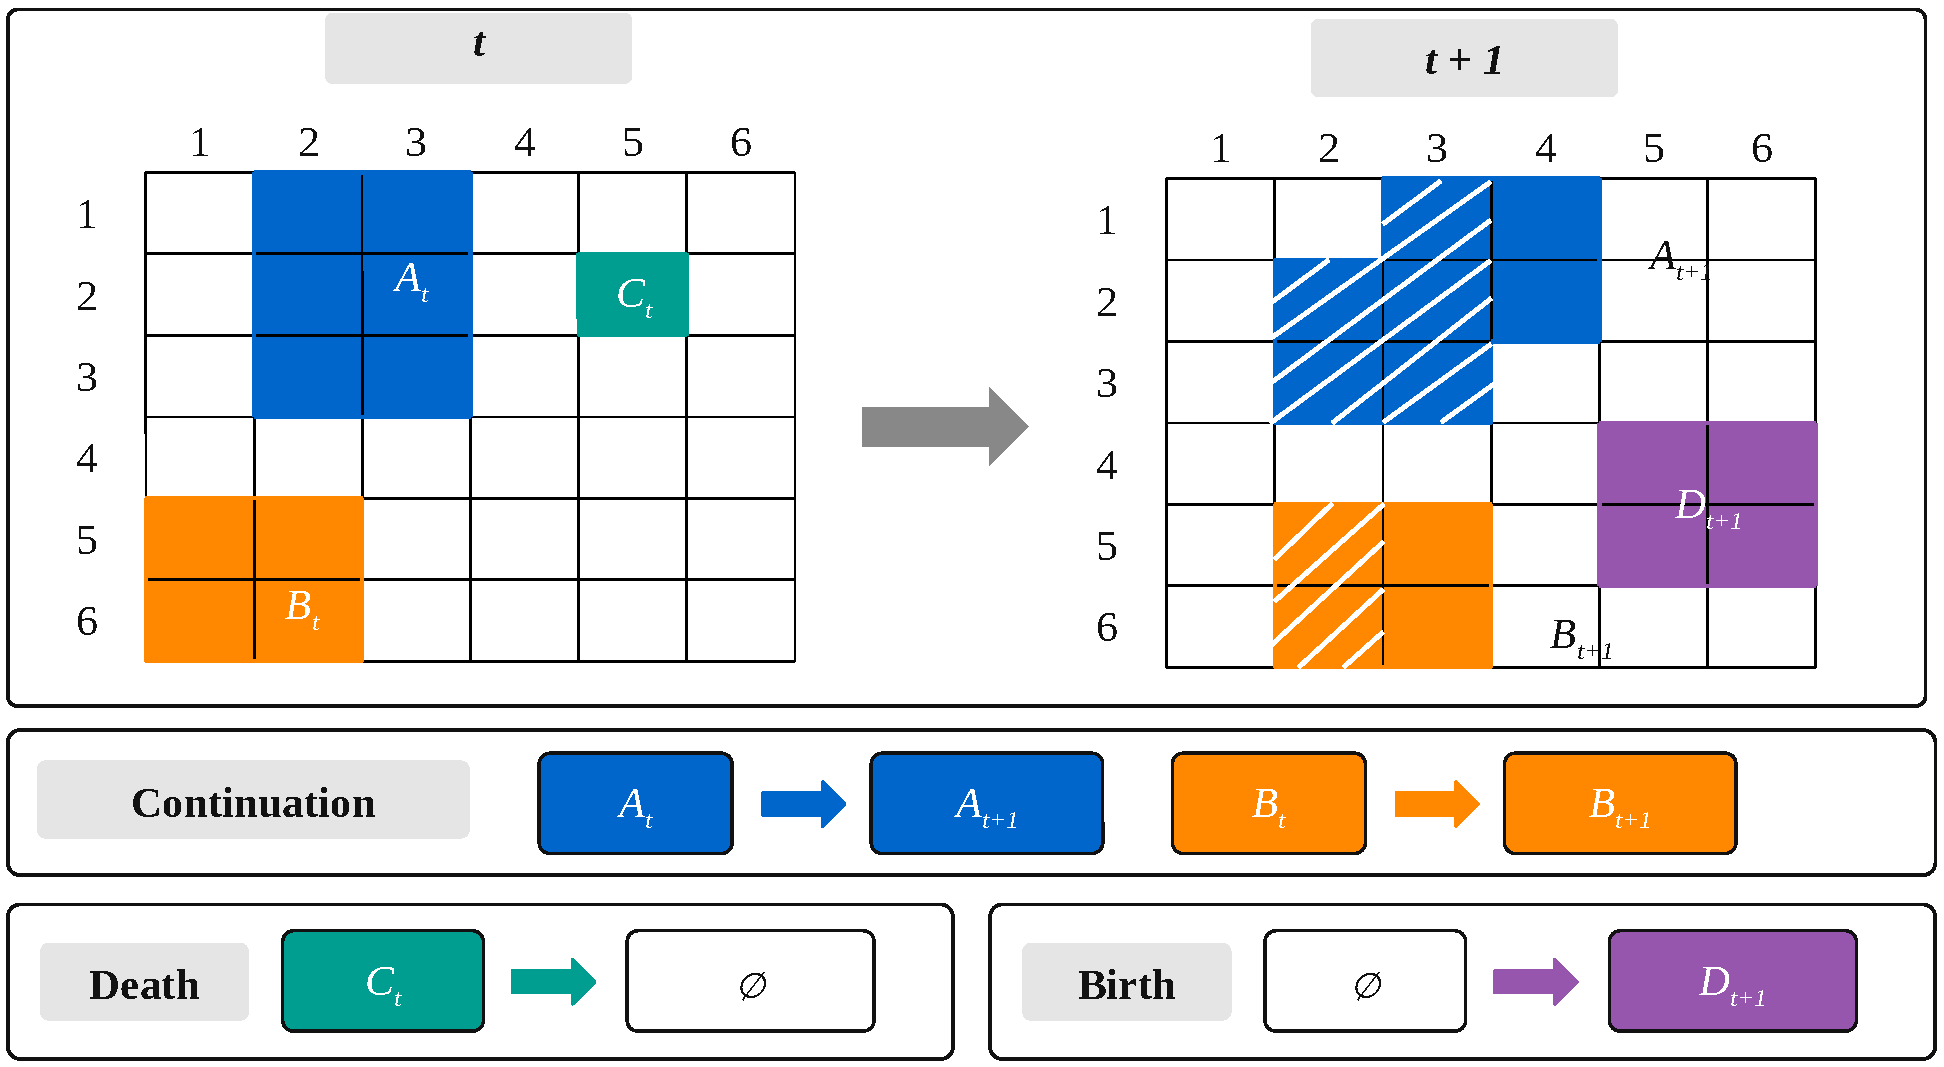
\includegraphics[width=\linewidth]{figures/anchor_leaf_correspondence.pdf}
\caption{Matching leaf-arc supports by one-to-one maximum overlap continues tracks across frames; unmatched leaves begin or end tracks. These correspondences supply the reference-motion samples.}
\label{fig:leaf_correspondence}
\end{figure}
The default direction maximizes squared matched-extremum motion:
\begin{equation}\label{eq:autodirection}
a^*\in\arg\max_{\|a\|=1}a^\top\Bigl(\sum_{t,i}\Delta p_i^t(\Delta p_i^t)^\top\Bigr)a,
\end{equation}
where $\Delta p_i^t=p_i^t-p_{\mu_t(i)}^{t-1}$ over valid links. Its sign makes total projected motion nonnegative; the longest domain axis handles zero motion energy. An analyst may supply a physical direction instead. For nearly zero signed motion, the largest-magnitude direction component is made positive; repeated leading eigenvalues can be resolved using a chosen physical axis. This separates reference estimation from the layout search: a budget changes the admissible map, while the coordinate being approximated stays fixed. Projected domain corners define one origin $o$ and extent $L$, giving
\begin{equation}\label{eq:reference}
q_i^t=\langle a^*,p_i^t\rangle-o\in[0,L].
\end{equation}
Direction, origin and extent remain fixed across frames and budgets. Relative geometry uses support-centroid distances $d_{ij}^t$; the targets $q_i^t$ use extremum locations. Thus support growth can change relative-distance terms without moving a feature's spatial target.

\subsection{A Unified Layout Formulation}\label{sec:common}
Each leaf occupies an interval of width $W_i=s\,m_i$ and center $z_i$, where $m_i$ is its support measure and $s$ is fixed. The layout set $\mathcal{L}(\pi;W)$ places these intervals in order $\pi$ inside $[0,L]$, with gap at least $g$ and anchor slack $|x_i-z_i|\le\rho W_i/2$. Two order costs distinguish point ordering from packing:
\begin{equation}\label{eq:nroe}
\begin{aligned}
\nroe(\pi)&=\frac{\max_{j\le k}[q_{\pi(j)}-q_{\pi(k)}]^+}{2L},\\
\tau(\pi)&=\min_{(x,z)\in\mathcal{L}(\pi;W)}\|x-q\|_\infty .
\end{aligned}
\end{equation}
NROE is the least normalized worst displacement of points in order $\pi$; $\tau$ includes the intervals and is an exactly solvable minimax linear program. Merge error measures the displayed hierarchy:
\begin{equation}\label{eq:dtop}
\dtop(\psi,T)=\max_{i,j}|V_{ij}^{\psi}-V_{ij}|\le\eta.
\end{equation}
The diagonal includes extremum values. Under complete fixed labelling this cophenetic error equals labelled interleaving distance and bounds the unlabelled interleaving and bottleneck distances~\cite{Munch:2019:LINF,Gasparovic:2024:IID,Morozov:2013:IDMT}.

These variables separate layout priorities in the common model
\begin{equation}\label{eq:family}
\begin{aligned}
\min_{\pi\in\Pi,\,(x,z)\in\mathcal{L}(\pi;W)}\;&\lambda_RE_R+\lambda_GE_G+\lambda_ME_M+\lambda_CE_C\\
\mathrm{s.t.}\;&\dtop\le\eta.
\end{aligned}
\end{equation}
where the terms fit spatial references, support distances, matched temporal targets and interval centers. TMTM packs tree-compatible blocks and aligns them by overlap; ST-MTM fits relative geometry with temporal constraints. Both preserve the tree and have no absolute-reference penalty. Anchoring adds $E_R$. \subsection{Conflict Between Topology and Spatial Position}
A projection can follow every $q_i$, but the order $A,C,D,B$ breaks the $A,B$ subtree block. The issue is the interaction between the spatial target order and the contiguous blocks required by a profile. Keeping those blocks may displace anchors; allowing some merge-level error may admit an order closer to the targets. This structural conflict precedes any choice of optimizer.

We address three questions: how much displacement exact topology forces (RQ1), how finite feature widths and interval constraints increase that cost (RQ2), and which conflicts can be released by bounded merge-level error (RQ3). The next section answers them in this order; the construction then uses the same quantities to select and place a map.

\section{The Positional Price of Keeping the Tree}\label{sec:bounds}
The positional cost comes from two sources: constraints imposed by the hierarchy and additional choices made by a layout. We first isolate the hierarchy in a point model, then account for interval packing, and finally allow controlled changes to merge levels. This progression answers RQ1--RQ3 using the same reference coordinate. Suppress $t$, write $[v]^+=\max(v,0)$ and take empty maxima as zero; complete packing derivations are in the supplementary material.

\subsection{Exact Topology}
The first question removes feature width and asks what the hierarchy alone forces. Exact topology keeps sibling subtrees in separate blocks, so their reference hulls determine the cost of choosing either block orientation. Let $[m_X,M_X]$ be the reference hull of subtree $X$ in the reduced equal-level tree.
\begin{theorem}[Exact-topology position bound]\label{thm:order}
Every exact profile satisfies $\nroe(\pi)\ge\nu^*$, where
\begin{equation}\label{eq:nu}
\nu^*=\frac{1}{2L}\max_v\max_{X\ne Y\in\mathrm{ch}(v)}[\min(M_X-m_Y,M_Y-m_X)]^+.
\end{equation}
Recursive ordering by child-hull midpoint attains $\nu^*$ in $O(n\log n)$ time.
\end{theorem}
Sibling blocks must take one orientation. Its inversion cost is either $[M_X-m_Y]^+/2$ or $[M_Y-m_X]^+/2$, and midpoint order chooses the smaller. Every inverted leaf pair separates at its LCA. Therefore error above $\nu^*$ can be removed by reordering in the point model.

\subsection{Finite Widths}
Set $H_i=\rho W_i/2$, $\ell_i=q_i-W_i/2-H_i$, $h_i=q_i+W_i/2+H_i$ and $s_i=W_i+g$. Packing summaries
\begin{equation}\label{eq:packing}
\begin{split}
A(S)&=\max_{a\in S}\bigl(\ell_a+\sum_{i\in S:\ell_i\ge\ell_a}s_i\bigr),\\
B(S)&=\max_{b\in S}\bigl(\sum_{i\in S:h_i\le h_b}s_i-h_b\bigr)
\end{split}
\end{equation}
measure the interval span forced by upper and lower reference-endpoint sets. Define $\omega(X,Y)=\tfrac12\min\{A(X)+B(Y),A(Y)+B(X)\}-g/2$, and $E_\partial=\max\{0,B(\mathcal F)-g,A(\mathcal F)-g-L\}$ for all leaves $\mathcal F$.
\begin{theorem}[Width-aware position bound]\label{thm:width}
For every feasible exact-topology interval layout,
\begin{equation}\label{eq:widthbound}
\|x-q\|_\infty\ge\tau(\pi)\ge\mathcal B_w
=\max\{E_\partial,\max_{(X,Y)\in\mathcal P_0}\omega(X,Y)\},
\end{equation}
where $\mathcal P_0$ contains distinct sibling descendant-leaf sets. With zero widths and gaps, $\mathcal B_w=L\nu^*$.
\end{theorem}
The first and last anchors must accommodate their intervals and intervening gaps up to the permitted anchor slack. Sibling contiguity chooses a block orientation, while the canvas ends supply $E_\partial$. Thus ordering alone no longer determines the positional cost: even an order attaining the point bound may require additional displacement to fit its intervals. The bound has coordinate units, while $\nu^*$ is normalized by $L$. This motivates evaluating the exact packing cost of each candidate order before optimizing its anchors.

\subsection{Bounded Merge Error}
If leaf $k$ lies between descendants $i,j$ of node $u$, interval containment gives $V_{ik}^{\psi}\le V_{ij}^{\psi}$, hence $V_{ik}\le h(u)+2\eta$. Let $A_\eta(u)$ be the highest ancestor with $h(A_\eta(u))-h(u)\le2\eta$. Form $\mathcal P_\eta$ from pairs $(\mathcal D(u),\{k\})$ with $k\notin\mathcal D(A_\eta(u))$, and pairs $(\mathcal D(u),\mathcal D(w))$ with each set disjoint from the other's $A_\eta$ ancestor set, for internal $u,w$.
\begin{theorem}[Bounded-topology position bound]\label{thm:chain}
If $\dtop\le\eta$, every pair in $\mathcal P_\eta$ lies wholly in one block orientation. Thus
\begin{equation}\label{eq:chainbounds}
\begin{split}
\nroe(\pi)&\ge C_\eta=\max_{(X,Y)\in\mathcal P_\eta}\frac{[\min(M_X-m_Y,M_Y-m_X)]^+}{2L},\\
\tau(\pi)&\ge C_{w,\eta}=\max\{E_\partial,\max_{(X,Y)\in\mathcal P_\eta}\omega(X,Y)\}.
\end{split}
\end{equation}
\end{theorem}
The accumulated ancestor gap determines which outside leaves may enter a block, so an allowance releases only the conflicts supported by sufficiently small merge-level differences. Flattening parent gaps of at most $2\eta$ gives a second certificate; we use the larger of the two valid bounds. Together, the three results distinguish forced displacement from displacement chosen by a layout. Their algorithmic implication is to search orders using the exact fixed-order cost $\tau$, admit them only when their merge error fits the allowance, and limit additional displacement during anchor placement. A certificate is a lower bound; the construction must still produce and check a feasible map.

\begin{figure*}[!tb]
\paperfigure{figures/anchor_framework.pdf}{fig:framework}{Schematic AnchorMTM workflow: extraction and referencing, topology-budgeted layout, and topology-to-1D reconstruction produce the temporal map. The layout panel combines leaf-order search and anchor placement.}
\end{figure*}
\section{AnchorMTM}\label{sec:method}\label{sec:construction}

Figure~\ref{fig:framework} summarizes the construction; its topology-budgeted layout panel contains the separate order-search and anchor-placement stages. Extract and Reference prepares the trees, identities and fixed targets defined in Section~\ref{sec:formulation}. Search Leaf Orders chooses an admissible order with low $\tau$. Place Anchors balances spatial and temporal objectives within a cap on that order's displacement. Reconstruct and Assemble builds the scalar profiles and stacks them along time. The output of each stage fixes the constraints passed to the next. The control is a normalized merge allowance $\varepsilon$, with $\eta=(\varepsilon_0+\varepsilon)\Delta_F$ for sequence scalar range $\Delta_F$ and numerical tolerance $\varepsilon_0=10^{-7}$. Exact Mode sets $\varepsilon=0$; the exact experiments use zero labelled error. Budgeted Mode uses a positive allowance within the same construction. Balanced denotes an experimentally selected positive-budget configuration, not all budgeted maps. Widths, gap, slack and weights stay fixed during a budget sweep; the merge allowance controls hierarchical error rather than directly bounding positional error.

\subsection{Order Selection and Optimal Barriers}
Order search receives the prepared tree, reference targets, widths and merge allowance. A finite candidate pool $\mathcal C$ starts from midpoint orders of the strict tree, threshold flattenings and selective conflict flattenings. Width-aware block moves refine promising structures. The point bound supplies an exact-topology initialization, while the interval analysis motivates evaluating packing displacement. Each visited order is checked against the original merge matrix, and selection is lexicographic:
\begin{equation}\label{eq:orderobjective}
\pi^\varepsilon\in\arg\min_{\pi\in\mathcal C}\bigl(\tau(\pi),\nroe(\pi)\bigr)
\quad\mathrm{s.t.}\quad\delta^*(\pi)\le\eta.
\end{equation}
The exact tree supplies a feasible strict-topology seed. Selective flattening releases additional permutations while retaining deeper blocks, as illustrated in Fig.~\ref{fig:selective_relaxation}.

\paragraph{Construction sequence.} For each frame, generate and refine candidate orders; compute $\tau$, NROE and $\delta^*$; admit the budget-feasible orders; choose the lexicographic minimum; solve its capped QP; fill and correct the profile; then check the rendered merge matrix and append the temporal column. The supplementary algorithm lists these steps with the tracking and rounding procedures.

\begin{figure}[!tb]
\centering
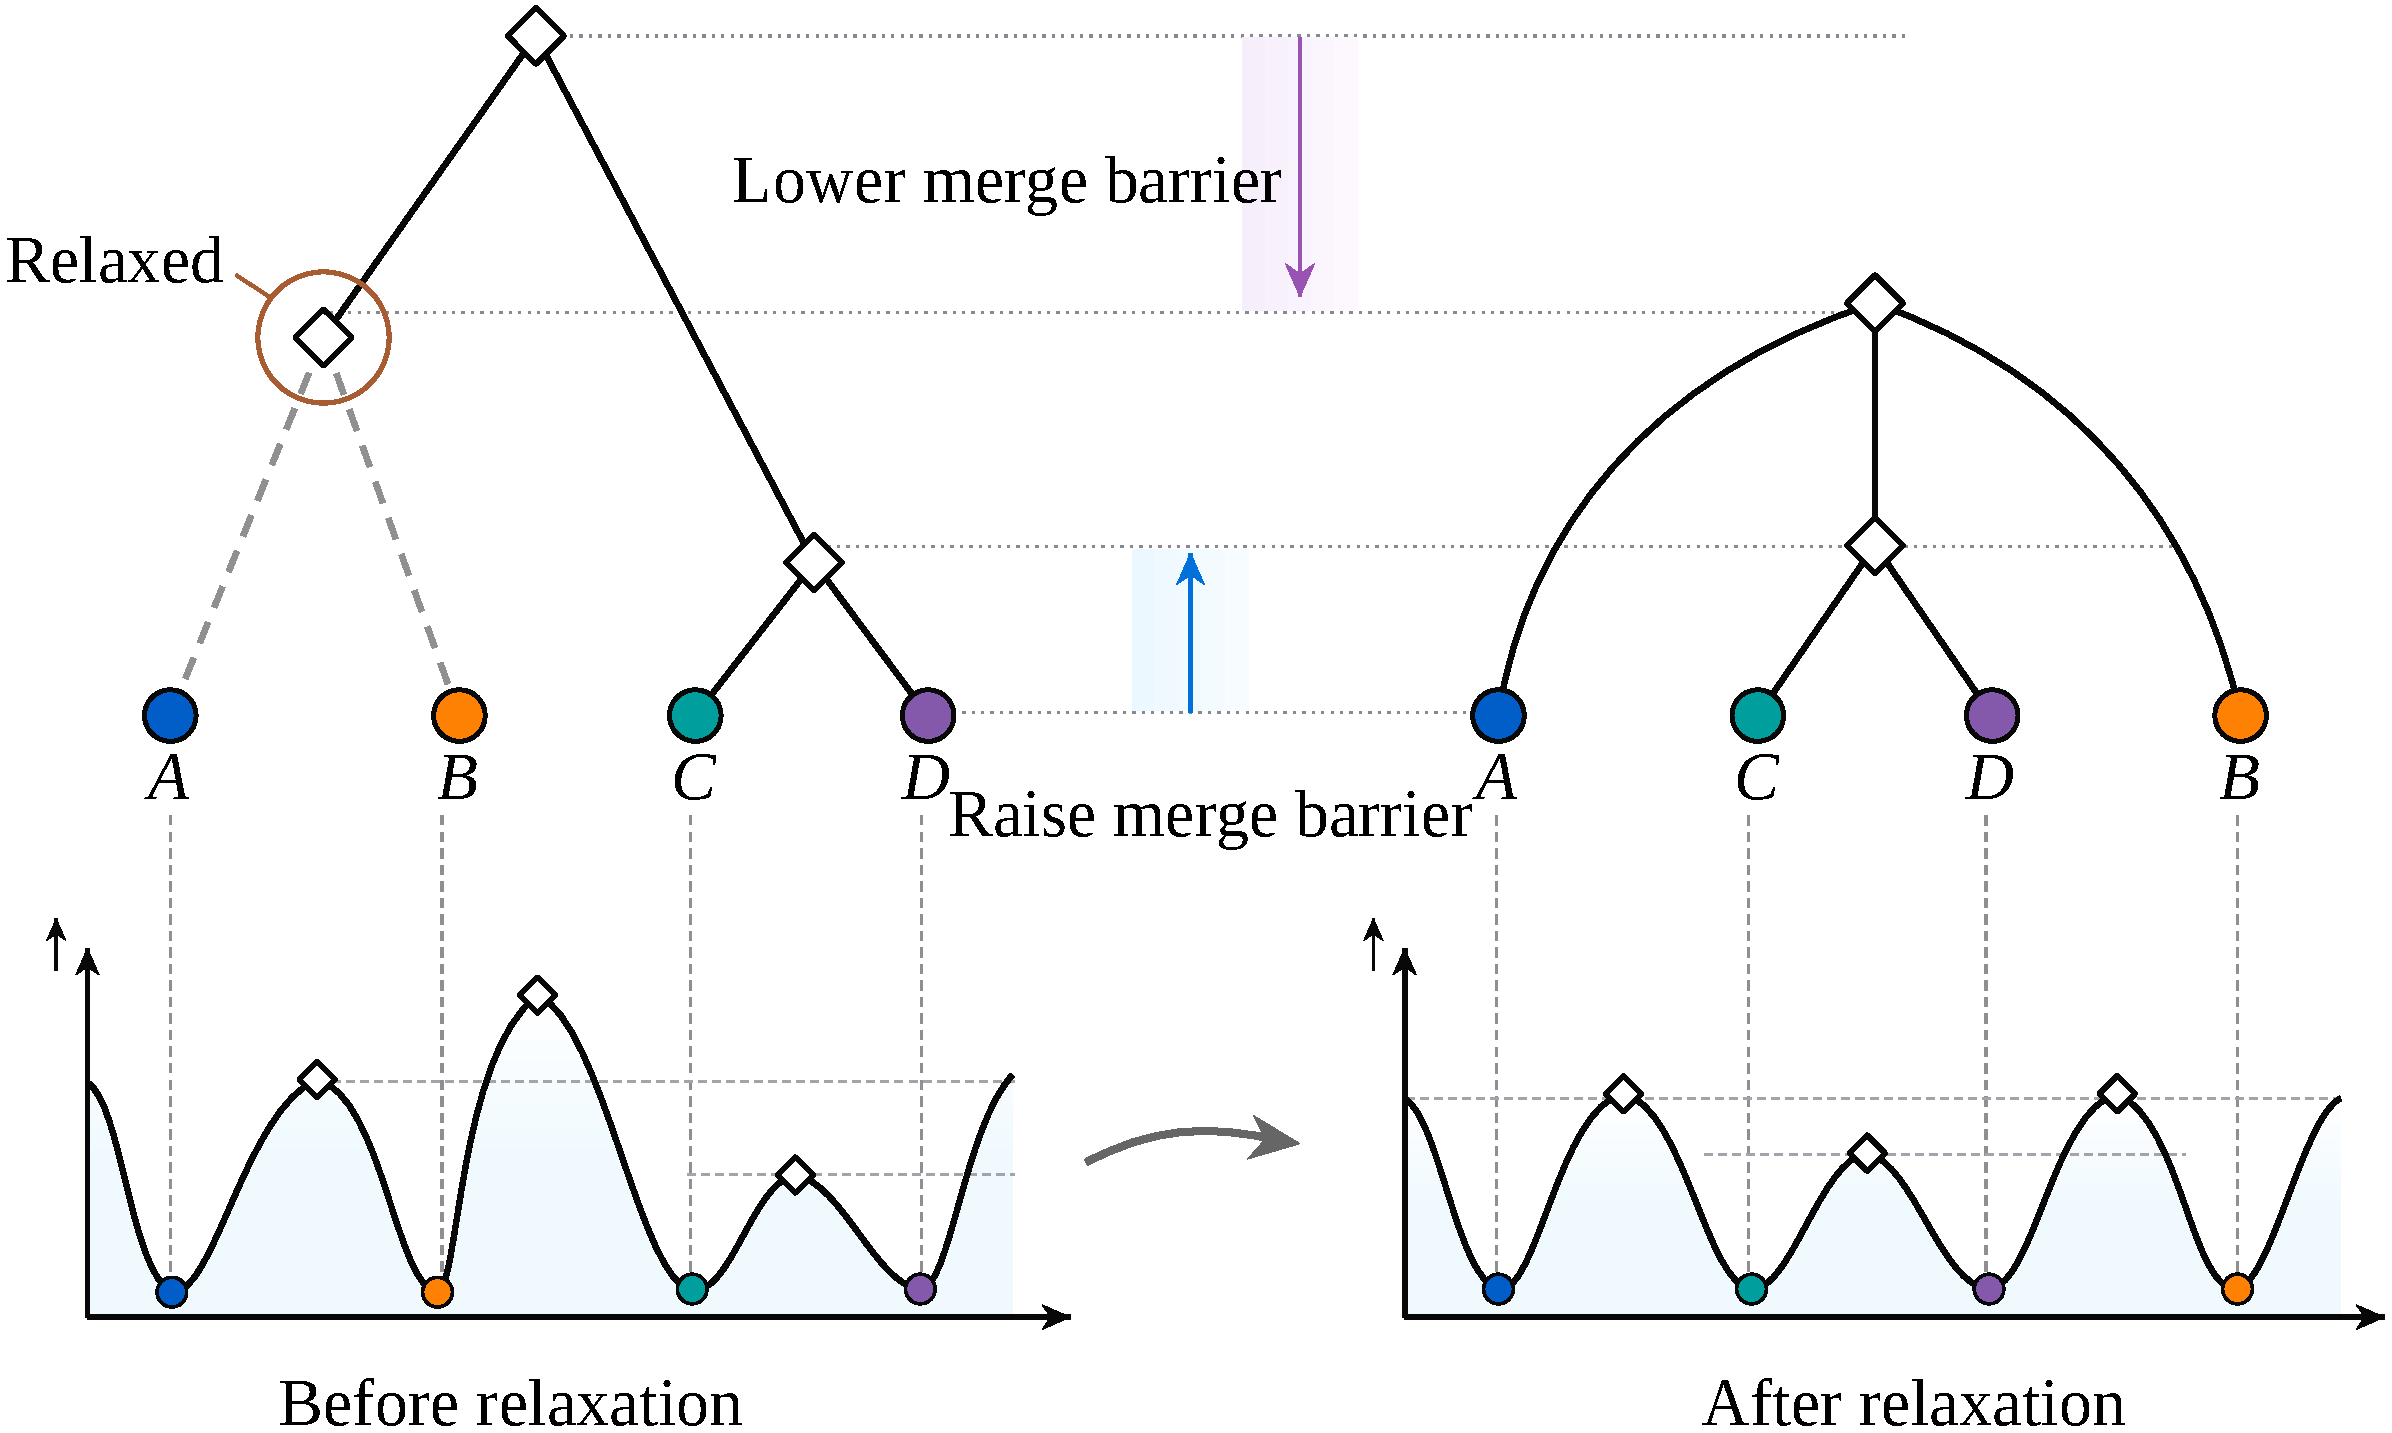
\includegraphics[width=\columnwidth]{figures/anchor_relaxation_open.pdf}
\caption{Selective flattening admits order $A,C,D,B$ while retaining the $C,D$ grouping. The displayed barrier levels are corrected against the original merge matrix.}
\label{fig:selective_relaxation}
\end{figure}
For gap $k$ of an order, set $C_k=\min_{i\le k<j}V_{\pi(i)\pi(j)}$ and let $F_k$ be the larger adjacent extremum value.
\begin{proposition}[Optimal barriers]\label{prop:barriers}
With fixed extrema, the least continuous merge error is
\begin{equation}\label{eq:delta}
\delta^*(\pi)=\max\Bigl\{0,\max_k(F_k-C_k),
\tfrac12\max_{i<j}\bigl(V_{\pi(i)\pi(j)}-\max_{i\le k<j}C_k\bigr)\Bigr\},
\end{equation}
attained by $b_k=C_k+\delta^*(\pi)$.
\end{proposition}
Indeed, error $\delta$ requires $F_k\le b_k\le C_k+\delta$; choosing the largest permitted barriers meets every pair's lower requirement exactly when $\delta\ge\delta^*$. This gives a closed-form admission test for candidate orders.

\subsection{Capped Spatiotemporal Placement}
For the chosen order, the default weights are $(\lambda_R,\lambda_G,\lambda_M,\lambda_C)=(4,1,0.5,0.1)$. Each term in Eq.~\ref{eq:family} is a mean squared residual: anchor-to-reference distance, ordered anchor separation minus support-centroid distance, matched temporal-target error, or anchor-to-center offset. The temporal target follows projected motion:
\begin{equation}\label{eq:temporal_target}
\hat x_i^t=x_{\mu_t(i)}^{t-1}+q_i^t-q_{\mu_t(i)}^{t-1}.
\end{equation}
The selected order is now fixed, so placement changes coordinates without revisiting the discrete search. Unmatched leaves have no temporal penalty. Placement solves the convex quadratic objective under the interval constraints and
\begin{equation}\label{eq:qp}
\|x-q\|_\infty\le\tau(\pi^\varepsilon)+\beta_0,
\end{equation}
with fixed slack $\beta_0$. Because $\tau$ is attained, this cap is feasible and transfers the selected order's displacement control to the final anchors. The cap prevents a relative-distance or temporal term from moving an anchor arbitrarily far from its spatial target. Conversely, the fixed slack leaves room to improve these secondary relationships after the discrete order has been chosen. Within a frame the feasible set is linear and the objective quadratic; frame order enters only through matched predecessor targets.

\subsection{Profile Reconstruction}
The final stage receives the order, anchor intervals and optimal barriers. Leaf-arc samples fill the intervals and LCA paths fill their gaps~\cite{Koepp:2023:TMTM,STMTM:2026}. Barrier correction clips each inter-anchor interior to $b_k$ and raises its peak when needed. Profiles share direction, origin, extent and pixel scale; their stack is $I^\varepsilon(t,u)=\psi_t^\varepsilon(u)$. Integer rounding can affect merge levels, so the rendered fixed-label matrix, including its diagonal, is checked after reconstruction. The supplementary material supplies the full algorithm and rounding procedure.

\begin{table*}[!tb]
\caption{Five-dataset comparison. Bold/underline mark best/second distinct values among comparable local measurements only; ties share emphasis. Daggered SNS/TW values are published context and excluded from ranking. Curves use fixed default orientations.}
\label{tab:quantitative-final}
\footnotesize
\setlength{\tabcolsep}{1.5pt}
\renewcommand{\arraystretch}{0.85}
\begin{tabular*}{\textwidth}{@{\extracolsep{\fill}}l*{12}{c}lccc@{}}
\toprule
\multirow{2}{*}{Dataset} & \multicolumn{3}{c}{Hilbert} & \multicolumn{3}{c}{Morton} & \multicolumn{3}{c}{TMTM} & \multicolumn{3}{c}{ST-MTM} & \multicolumn{4}{c}{AnchorMTM (ours)} \\
\cmidrule(lr){2-4}\cmidrule(lr){5-7}\cmidrule(lr){8-10}\cmidrule(lr){11-13}\cmidrule(lr){14-17}
 & SNS$\downarrow$ & TW$\uparrow$ & NPE$\downarrow$ & SNS$\downarrow$ & TW$\uparrow$ & NPE$\downarrow$ & SNS$\downarrow$ & TW$\uparrow$ & NPE$\downarrow$ & SNS$\downarrow$ & TW$\uparrow$ & NPE$\downarrow$ & Mode & SNS$\downarrow$ & TW$\uparrow$ & NPE$\downarrow$ \\
\midrule
\multirow{2}{*}{Gaussian} & \multirow{2}{*}{$0.1117$} & \multirow{2}{*}{$0.6719$} & \multirow{2}{*}{$0.7557$} & \multirow{2}{*}{$\underline{0.0393}$} & \multirow{2}{*}{$\underline{0.8333}$} & \multirow{2}{*}{$0.7359$} & \multirow{2}{*}{$0.25^{\dagger}$} & \multirow{2}{*}{$0.77^{\dagger}$} & \multirow{2}{*}{$\underline{0.1118}$} & \multirow{2}{*}{$0.06^{\dagger}$} & \multirow{2}{*}{$1.00^{\dagger}$} & \multirow{2}{*}{$0.1154$} & Exact & $\mathbf{0.0353}$ & $\mathbf{0.9323}$ & $\mathbf{0.0089}$ \\
 &  &  &  &  &  &  &  &  &  &  &  &  & Balanced & $\mathbf{0.0353}$ & $\mathbf{0.9323}$ & $\mathbf{0.0089}$ \\
\multirow{2}{*}{Ring} & \multirow{2}{*}{$\mathbf{0.1252}$} & \multirow{2}{*}{$\mathbf{0.9048}$} & \multirow{2}{*}{$0.5941$} & \multirow{2}{*}{$0.1489$} & \multirow{2}{*}{$0.7619$} & \multirow{2}{*}{$0.6033$} & \multirow{2}{*}{$0.28^{\dagger}$} & \multirow{2}{*}{$0.68^{\dagger}$} & \multirow{2}{*}{$0.1756$} & \multirow{2}{*}{$0.21^{\dagger}$} & \multirow{2}{*}{$0.88^{\dagger}$} & \multirow{2}{*}{$0.2463$} & Exact & $0.1485$ & $\underline{0.8571}$ & $\underline{0.0471}$ \\
 &  &  &  &  &  &  &  &  &  &  &  &  & Balanced & $\underline{0.1334}$ & $\underline{0.8571}$ & $\mathbf{0.0395}$ \\
\multirow{2}{*}{Wildfires} & \multirow{2}{*}{$0.1883$} & \multirow{2}{*}{$0.8303$} & \multirow{2}{*}{$0.3641$} & \multirow{2}{*}{$0.1304$} & \multirow{2}{*}{$0.8758$} & \multirow{2}{*}{$0.1560$} & \multirow{2}{*}{$0.44^{\dagger}$} & \multirow{2}{*}{$0.88^{\dagger}$} & \multirow{2}{*}{$0.2280$} & \multirow{2}{*}{$0.24^{\dagger}$} & \multirow{2}{*}{$0.91^{\dagger}$} & \multirow{2}{*}{$0.3180$} & Exact & $\mathbf{0.0426}$ & $\mathbf{0.9136}$ & $\underline{0.0131}$ \\
 &  &  &  &  &  &  &  &  &  &  &  &  & Balanced & $\underline{0.0447}$ & $\underline{0.8989}$ & $\mathbf{0.0116}$ \\
\multirow{2}{*}{Storms} & \multirow{2}{*}{$0.1290$} & \multirow{2}{*}{$0.7403$} & \multirow{2}{*}{$0.3705$} & \multirow{2}{*}{$0.1180$} & \multirow{2}{*}{$0.7251$} & \multirow{2}{*}{$0.3468$} & \multirow{2}{*}{$0.34^{\dagger}$} & \multirow{2}{*}{$0.71^{\dagger}$} & \multirow{2}{*}{$0.5753$} & \multirow{2}{*}{$0.21^{\dagger}$} & \multirow{2}{*}{$0.94^{\dagger}$} & \multirow{2}{*}{$0.4579$} & Exact & $\underline{0.0790}$ & $\underline{0.8463}$ & $\underline{0.0399}$ \\
 &  &  &  &  &  &  &  &  &  &  &  &  & Balanced & $\mathbf{0.0743}$ & $\mathbf{0.8766}$ & $\mathbf{0.0140}$ \\
\multirow{2}{*}{PM2.5} & \multirow{2}{*}{$0.2386$} & \multirow{2}{*}{$\mathbf{0.8887}$} & \multirow{2}{*}{$0.8090$} & \multirow{2}{*}{$\underline{0.1760}$} & \multirow{2}{*}{$\underline{0.8277}$} & \multirow{2}{*}{$0.8823$} & \multirow{2}{*}{$0.3018$} & \multirow{2}{*}{$0.7781$} & \multirow{2}{*}{$0.5241$} & \multirow{2}{*}{$0.1897$} & \multirow{2}{*}{$0.8224$} & \multirow{2}{*}{$0.5577$} & Exact & $0.1964$ & $0.7884$ & $\underline{0.1390}$ \\
 &  &  &  &  &  &  &  &  &  &  &  &  & Balanced & $\mathbf{0.1636}$ & $0.7657$ & $\mathbf{0.0468}$ \\
\bottomrule
\end{tabular*}
\vspace{2pt}
\begin{minipage}{\textwidth}\footnotesize For the original four inputs, TMTM/ST-MTM Temporal SNS/TW ($\dagger$) are published values; other entries are local measurements. Author inputs and coverage are unconfirmed. Local TW coverage (Gaussian/Ring/Wildfires/Storms) is 64/64, 1/40, 4/32, 11/744; ineligible frames are omitted. Published TW has two-decimal precision. Mode applies only to AnchorMTM. PM2.5 uses 744 shared-input local frames (TW $k=1$, full coverage); its Balanced mode uses the fixed exploratory 5\% case budget, without validation-set budget selection. ST-MTM uses the Storms preset with start frame 0; PM2.5 baseline metrics are all recomputed.\end{minipage}

\end{table*}
\begin{figure*}[!tb]
\paperfigure[.94\textwidth]{figures/volume_gallery.pdf}{fig:volume-gallery}{Recomputed feature positions on Tangaroa and Cylinder using the default-weight volume configuration. Grey reference points and signed-displacement colors connect feature positions to $q$. Each panel reports the feature-pooled mean absolute displacement and NPE (mean per-frame maximum); positive budgets also report maximum attained merge error. Baseline reflection minimizes pooled reference displacement. These runs use the fixed configurations described in the protocol, distinct from the selected geometry-oriented table settings.}
\end{figure*}


\section{Experiments}\label{sec:experiments}
The evidence follows the argument developed above: validate the positional restrictions, measure absolute spatial positioning, then examine how a merge allowance changes displacement. We first establish the data and comparison protocol, use controlled and real trees to test the bounds, and connect the quantitative results to complete temporal maps and their source fields.

\subsection{Experimental Setup}
Five planar inputs are Gaussian (64 frames), Ring (40), Wildfires (32), Storms (744) and hourly PM2.5 (744). The first four use per-frame persistence fractions $(0.001,0.001,0.15,0.105)$ following the ST-MTM benchmark~\cite{STMTM:2026}. They are local reconstructions: three Gaussian peaks, the archived Ring generator, aggregated wildfire radiative power and ERA5 pressure anomalies. PM2.5 interpolates the January 2017 CAQRA hourly fields to a $160\times144$ grid, with 5\% per-frame persistence. Raster lengths are 4096, except Ring's original 196 positions.

The volumes are Cylinder (102 cropped $135\times64\times48$ $Q$-criterion fields, 2\% per-frame persistence)~\cite{Camarri:2005:Cylinder,Weinkauf:SquareCylinder} and Tangaroa (201 $300\times180\times120$ speed fields, range $[0,2]$, absolute persistence 0.2)~\cite{Popinet:2004:Tangaroa}. Within each comparison, methods share fields, retained labels and support geometry.

SNS measures scale-normalized support-distance stress~\cite{Smelser:2025:Scale}; TW measures neighborhood preservation~\cite{Venna:2001:NP}. Absolute positioning uses
\begin{equation}\label{eq:experimental-npe}
\mathrm{NPE}=\frac1T\sum_t\frac{\max_i|x_i^t-q_i^t|}{L}.
\end{equation}
For the original four planar inputs, published TMTM/ST-MTM SNS/TW provide context (daggers in Table~\ref{tab:quantitative-final}); NPE is measured locally. Local TW coverage is 64/64, 1/40, 4/32 and 11/744 for $k=(1,3,5,3)$. PM2.5 and volume scores are all local, with $k=1$ and full coverage. For PM2.5, the first frame with nonconstant anchors and references determines one sequence-wide reflection from the sign of their covariance: TMTM is reflected and ST-MTM is not. Hilbert/Morton use fixed orientations and full-grid ranks. Thus NPE compares a common reference, while SNS/TW evaluate complementary spatial relationships.

Exact uses zero allowance. On the four benchmark inputs, Balanced selects a positive budget from 1--10\% on the first chronological quarter by minimizing the equal-weight normalized NPE/SNS score, with smaller budgets breaking near ties; the resulting budgets are 1, 1, 5 and 10\%. PM2.5 retains its fixed 5\% mode. Sequence-level references and full-sequence reporting include these selection frames. Volume tables use fixed $+x$ references and selected geometry-oriented configurations; their complete parameters are in the supplement. The volume position/distribution figures use a second, common default-weight configuration, with motion-derived direction for Tangaroa and $x$ for Cylinder.

\begin{figure*}[!t]
\paperfigure[.90\textwidth]{figures/budget_distribution_complete.pdf}{fig:budget-distribution}{Recomputed per-frame budget response. Upper row: worst displacement, with quartiles, 5th--95th percentile whiskers, outliers and mean diamonds (square-root scale). Lower row: measured merge error and budget guides. Ring, Storms and PM2.5 use budgets 0, 1, 2, 5, 10 and 20\%; the two default-weight volumes use 0, 2, 5, 10 and 20\%. Orange marks the selected planar modes. Every plotted frame passes its continuous and raster budget checks.}
\end{figure*}
\subsection{Validation of Position Bounds}\label{sec:bounds-eval}

\begin{figure}[!tb]
\centering
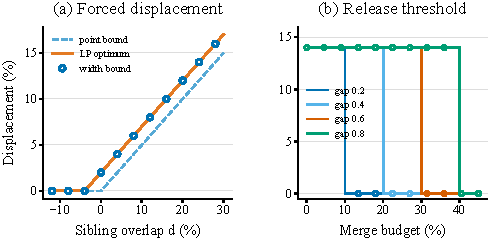
\includegraphics[width=\columnwidth]{figures/anchor_controlled_bounds.pdf}
\caption{Independent four-leaf validation. (a) The width-aware bound and order search coincide with exhaustive minimax LPs over 24 orders. (b) For four parent gaps, the displacement disappears when twice the merge allowance reaches that gap. Circles mark the recomputed bounds.}
\label{fig:controlled}
\end{figure}
To isolate the constraints in RQ1--RQ3, two sibling pairs merge below a root at 1, with leaf values 0 and targets $(0.2,0.5,0.5-d,0.8-d)$. Across 43 overlaps $d\in[-0.12,0.30]$, independent minimax LPs evaluate every leaf permutation. With width 0.06, gap 0.01 and $\rho=0.5$, the exhaustive optimum, width certificate and selected order coincide at $\tau=\max(0,(d+0.04)/2)$ (Fig.~\ref{fig:controlled}a). At $d=0.24$, the point cost is 12\% and the interval cost 14\%.

For parent gaps $h\in\{0.2,0.4,0.6,0.8\}$ and 91 budgets each, all 364 recomputed tests recover the release threshold $2\varepsilon=h$ (Fig.~\ref{fig:controlled}b). These tests connect the three bounds: interleaving causes the point obstruction, widths add packing, and scalar merge gaps determine the price of releasing a block.

\paragraph{Current data sequences.}
The same calculation applies to every frame of our five planar inputs. Table~\ref{tab:real-bounds} recomputes their bounds from the simplified source trees, extremum targets and fixed widths. The selected Exact order attains the width-aware bound on 1,335 of 1,624 frames. On those frames the certificate and an admissible solution coincide, establishing the optimum over all exact-topology orders. Gaussian and Ring attain it on every frame; Wildfires misses it on one and Storms on 15. PM2.5 attains it on 471 of 744 frames and leaves a larger residual gap: mean normalized $\tau$ is 13.11\%, versus a mean bound of 12.88\%. This is the interval-order cost before the capped placement objective chooses the final anchors.

The baseline columns of Table~\ref{tab:real-bounds} distinguish forced displacement from the additional point-order error introduced by each recorded layout. For each frame we sort its recorded anchors and evaluate NROE against the same $q$. The displayed share is $1-\sum_t\nu_t^*/\sum_t\nroe(\pi_t)$, so midpoint ordering removes that share without changing the tree in the point model. On Storms the excess is 91.0\% for TMTM and 83.0\% for ST-MTM; on PM2.5 it is 56.4\% and 59.7\%. The width certificate then identifies the packing cost that remains after order improvement. Together these measurements turn the distinction between forced and chosen displacement into a per-sequence diagnostic.
\begin{table}[!tb]
\centering\caption{Current planar sequences: Exact orders attaining the width-aware lower bound, and the share of local baseline point-order error above the exact point bound. Orientations match the primary measurements.}\label{tab:real-bounds}
\footnotesize\setlength{\tabcolsep}{3pt}
\begin{tabular}{@{}lrrcc@{}}\toprule
Dataset & Frames & Width hits & TMTM excess & ST-MTM excess\\\midrule
Gaussian & 64 & 64 & 100.0\% & 100.0\% \\
Ring & 40 & 40 & 64.5\% & 25.7\% \\
Wildfires & 32 & 31 & 92.5\% & 98.1\% \\
Storms & 744 & 729 & 91.0\% & 83.0\% \\
PM2.5 & 744 & 471 & 56.4\% & 59.7\% \\
\bottomrule\end{tabular}\end{table}

\begin{figure*}[!tb]
\paperfigure{figures/anchor_storms_budget_maps.pdf}{fig:storms-budget-profiles}{Storms event window, frames 355--460, at five AnchorMTM budgets and with local TMTM/ST-MTM maps on the same case-study fields and trees. Common crops and the $[-35,35]$ hPa scale connect the map trajectories to the reference feature.}
\end{figure*}
\subsection{Absolute Spatial Positioning}\label{sec:reference-results}

With the structural cost established, we evaluate the final anchors against the fixed reference. Balanced has lower NPE than the fixed curves and both local merge-tree adapters on all five planar inputs (Table~\ref{tab:quantitative-final}). Against curves, it also improves SNS and TW on Gaussian, Wildfires and Storms. Ring favors Hilbert's SNS/TW (0.1252/0.9048 versus 0.1334/0.8571), and PM2.5 favors Hilbert's TW (0.8887 versus 0.7657). The anchored axis improves location reading while retaining a different balance of local geometry.

\begin{table}[!tb]
\centering
\caption{Volumetric comparison with a fixed $x$ reference. Bold/underline mark best/second distinct values per dataset; ties share emphasis.}
\label{tab:volume-comparison}
\footnotesize
\setlength{\tabcolsep}{1.2pt}
\renewcommand{\arraystretch}{0.9}
\begin{tabular*}{\columnwidth}{@{\extracolsep{\fill}}lccc lccc@{}}
\toprule
\multirow{2}{*}{Dataset} & \multicolumn{3}{c}{TMTM} & \multicolumn{4}{c}{AnchorMTM (ours)} \\
\cmidrule(lr){2-4}\cmidrule(lr){5-8}
 & SNS$\downarrow$ & TW$\uparrow$ & NPE$\downarrow$ & Mode & SNS$\downarrow$ & TW$\uparrow$ & NPE$\downarrow$ \\
\midrule
\multirow{2}{*}{Cylinder} & \multirow{2}{*}{$0.2956$} & \multirow{2}{*}{$\underline{0.8017}$} & \multirow{2}{*}{$0.4769$} & Exact & $\underline{0.1226}$ & $0.8010$ & $\underline{0.1773}$ \\
 &  &  &  & Balanced & $\mathbf{0.0329}$ & $\mathbf{0.9117}$ & $\mathbf{0.0458}$ \\
\multirow{2}{*}{Tangaroa} & \multirow{2}{*}{$0.5255$} & \multirow{2}{*}{$0.6701$} & \multirow{2}{*}{$0.3866$} & Exact & $\underline{0.1204}$ & $\underline{0.8213}$ & $\underline{0.1285}$ \\
 &  &  &  & Balanced & $\mathbf{0.1124}$ & $\mathbf{0.8408}$ & $\mathbf{0.0653}$ \\
\bottomrule
\end{tabular*}
\vspace{2pt}
\begin{minipage}{\columnwidth}\footnotesize All values are local measurements, including adapted TMTM. TW uses $k=1$, with coverage 102/102 and 201/201. Mode applies only to AnchorMTM. Configurations are frozen exploratory results, not a blind test; settings appear in Table~\ref{tab:volume-parameters}.\end{minipage}
\end{table}

In the selected fixed-$x$ configurations, Balanced lowers SNS and NPE and raises TW relative to TMTM on both volumes (Table~\ref{tab:volume-comparison}). Cylinder NPE falls from 47.69\% to 4.58\%; Tangaroa falls from 38.66\% to 6.53\%. The selected Tangaroa configuration has zero reference weight and a 33.33\% allowance, so the mechanism is primarily geometry fitting within the prescribed reference cap.

Figure~\ref{fig:volume-gallery} reveals the spatial patterns behind reference error. Its default Exact configuration has NPE 11.18\% on Tangaroa and 9.18\% on Cylinder, versus TMTM's 30.63\% and 47.69\%. A 5\% budget brings Cylinder to 1.19\%, while Tangaroa reaches 8.91\% and needs 20\% to reach 1.88\%. The grey reference columns show the trajectories against which these displacements are measured.

\begin{figure*}[!tb]
\paperfigure{figures/anchor_cylinder_centered_blue.pdf}{fig:cylinder-centered}{Cylinder: a central-tree guidance variant and five source $Q$ isosurfaces, using a common camera and blue scalar scale. Stages I--V identify early, transition, shedding, transition and late configurations. Its ordinate expresses the guided layout position.}
\end{figure*}
\subsection{Position--Topology Trade-off}\label{sec:relaxation-results}
We next hold the prepared sequence and layout settings fixed and vary the merge allowance. The primary Exact planar runs have zero fixed-leaf merge error. Balanced attains maximum normalized errors 0, 0.982\%, 4.421\% and 9.985\% on Gaussian, Ring, Wildfires and Storms, within their declared budgets. Relative to Exact, NPE decreases by 16.2\%, 11.6\% and 64.9\% on the latter three inputs; Gaussian remains unchanged. Wildfires SNS rises from 0.0426 to 0.0447, showing that improved anchoring can change relative geometry in the other direction.

Figure~\ref{fig:budget-distribution} localizes this improvement. On Storms, a 10\% allowance changes the median displacement from 1.10\% to 0.84\%, but lowers the 90th percentile from 10.7\% to 2.5\%; 482 of 744 frames retain zero merge error. The budget therefore acts chiefly on a difficult tail: its main benefit is concentrated in frames with larger reference conflicts. In the default volumes, 200 of 201 Tangaroa frames and 98 of 102 Cylinder frames use a positive allowance, shifting most of the distribution.

The completed PM2.5 sweep uses the same input, tracks, reference, widths and weights at all six budgets. Its NPE decreases through 13.90\%, 10.30\%, 8.33\%, 4.68\%, 2.15\% and 1.15\%. All 2,976 newly solved frames at 1, 2, 10 and 20\% pass continuous and raster checks. TW changes from 0.7884 in Exact to 0.7580 at 20\%, linking the anchoring gain to a neighborhood cost.

\subsection{Case Studies}

The preceding measurements quantify reference alignment and the effect of the budget. The following cases connect those changes to scalar profiles, spatial snapshots and the coordinate each configuration is designed to show.

\paragraph{Storms.} The case-study preprocessing of Fig.~\ref{fig:storms_overview} supplies the common fields for Fig.~\ref{fig:storms-budget-profiles}. The 0, 2 and 5\% maps overlap locally; 10 and 20\% move the selected feature toward its reference. TMTM aligns subtrees by overlap, while ST-MTM fits relative geometry with temporal constraints. The common event window lets the reader follow the resulting trajectory differences.

\paragraph{Cylinder.}\label{sec:centered-volume} Central-tree guidance adds $16\,\mathrm{mean}_i(x_i-g_i)^2$ to the placement objective and reveals unfolding in Fig.~\ref{fig:cylinder-centered}. A 1\% allowance and 56.21\% position cap yield zero measured retained-leaf merge error. The snapshots at $t=32.1$, 56.1, 80.2, 120.3 and 162.0 link the five visual stages to the three-dimensional structures. This guidance changes the coordinate's role: frame-balanced absolute $X$ error rises from 21.1\% to 28.1\% as its weight grows from 1 to 16, trading location accuracy for hierarchical unfolding.

\begin{figure}[!tb]
\centering
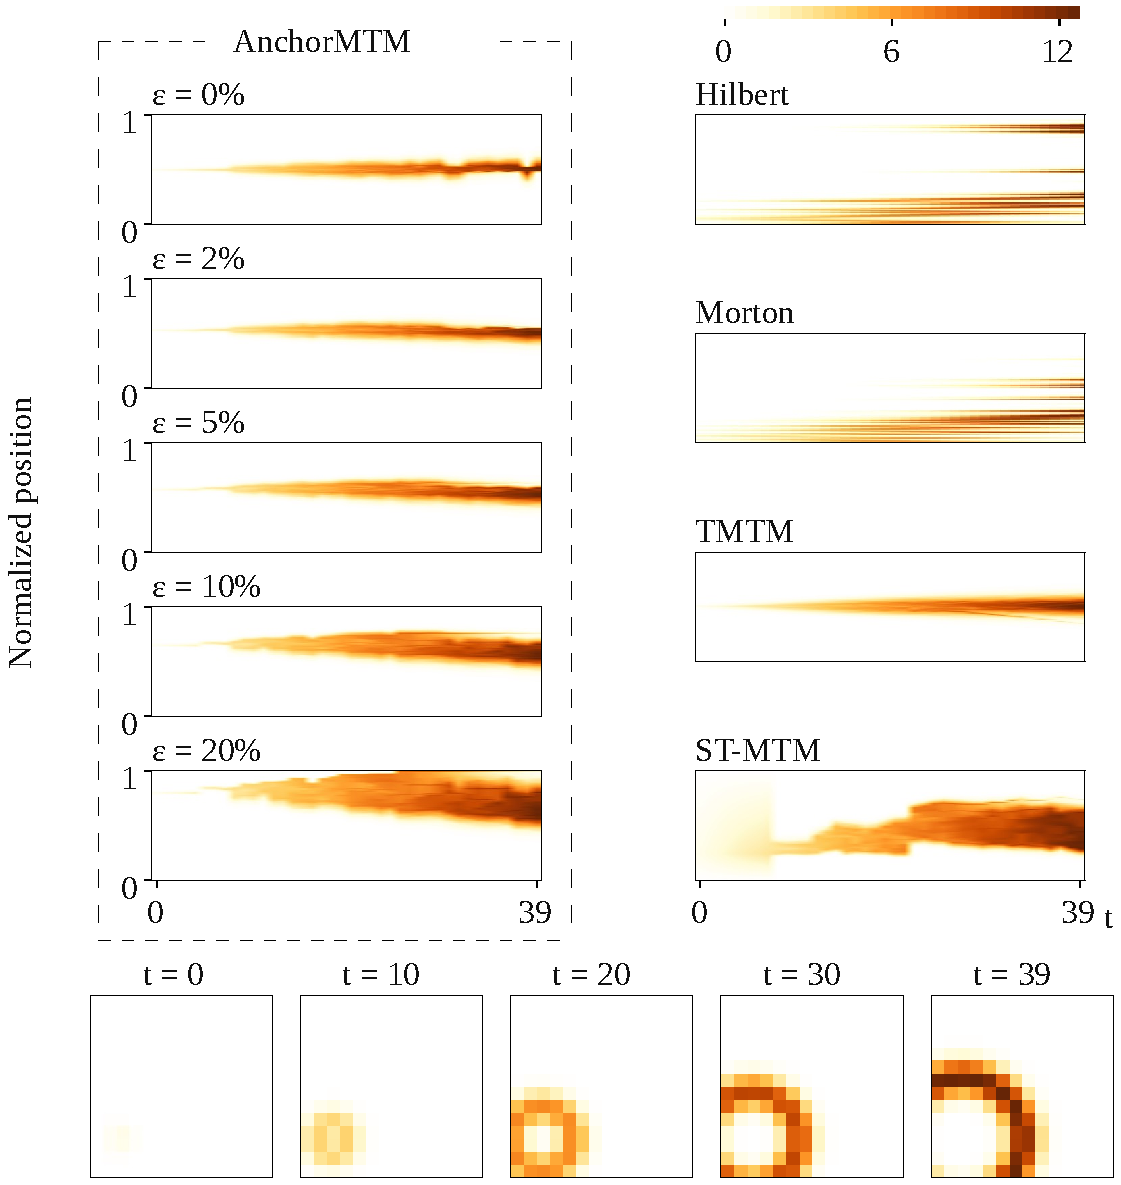
\includegraphics[width=\columnwidth]{figures/anchor_ring_result.pdf}
\caption{Ring: joint spatial guidance and merge allowances 0, 2, 5, 10 and 20\%, with same-input TMTM/ST-MTM maps, supplied curve panels and five source snapshots. All computed maps retain 40 frames and 196 positions.}
\label{fig:ring-result}
\end{figure}
\paragraph{Ring.} Figure~\ref{fig:ring-result} varies guidance jointly with budget: $q_{layout}=(1-\alpha)q_{mid}+\alpha q_{physical}$, with $\alpha=\varepsilon/20\%$ and a fixed $-128.7^\circ$ physical direction. Increasing guidance moves the ring toward its projected positions; the snapshots connect this change to expansion and strengthening.

\begin{figure}[!tb]
\centering
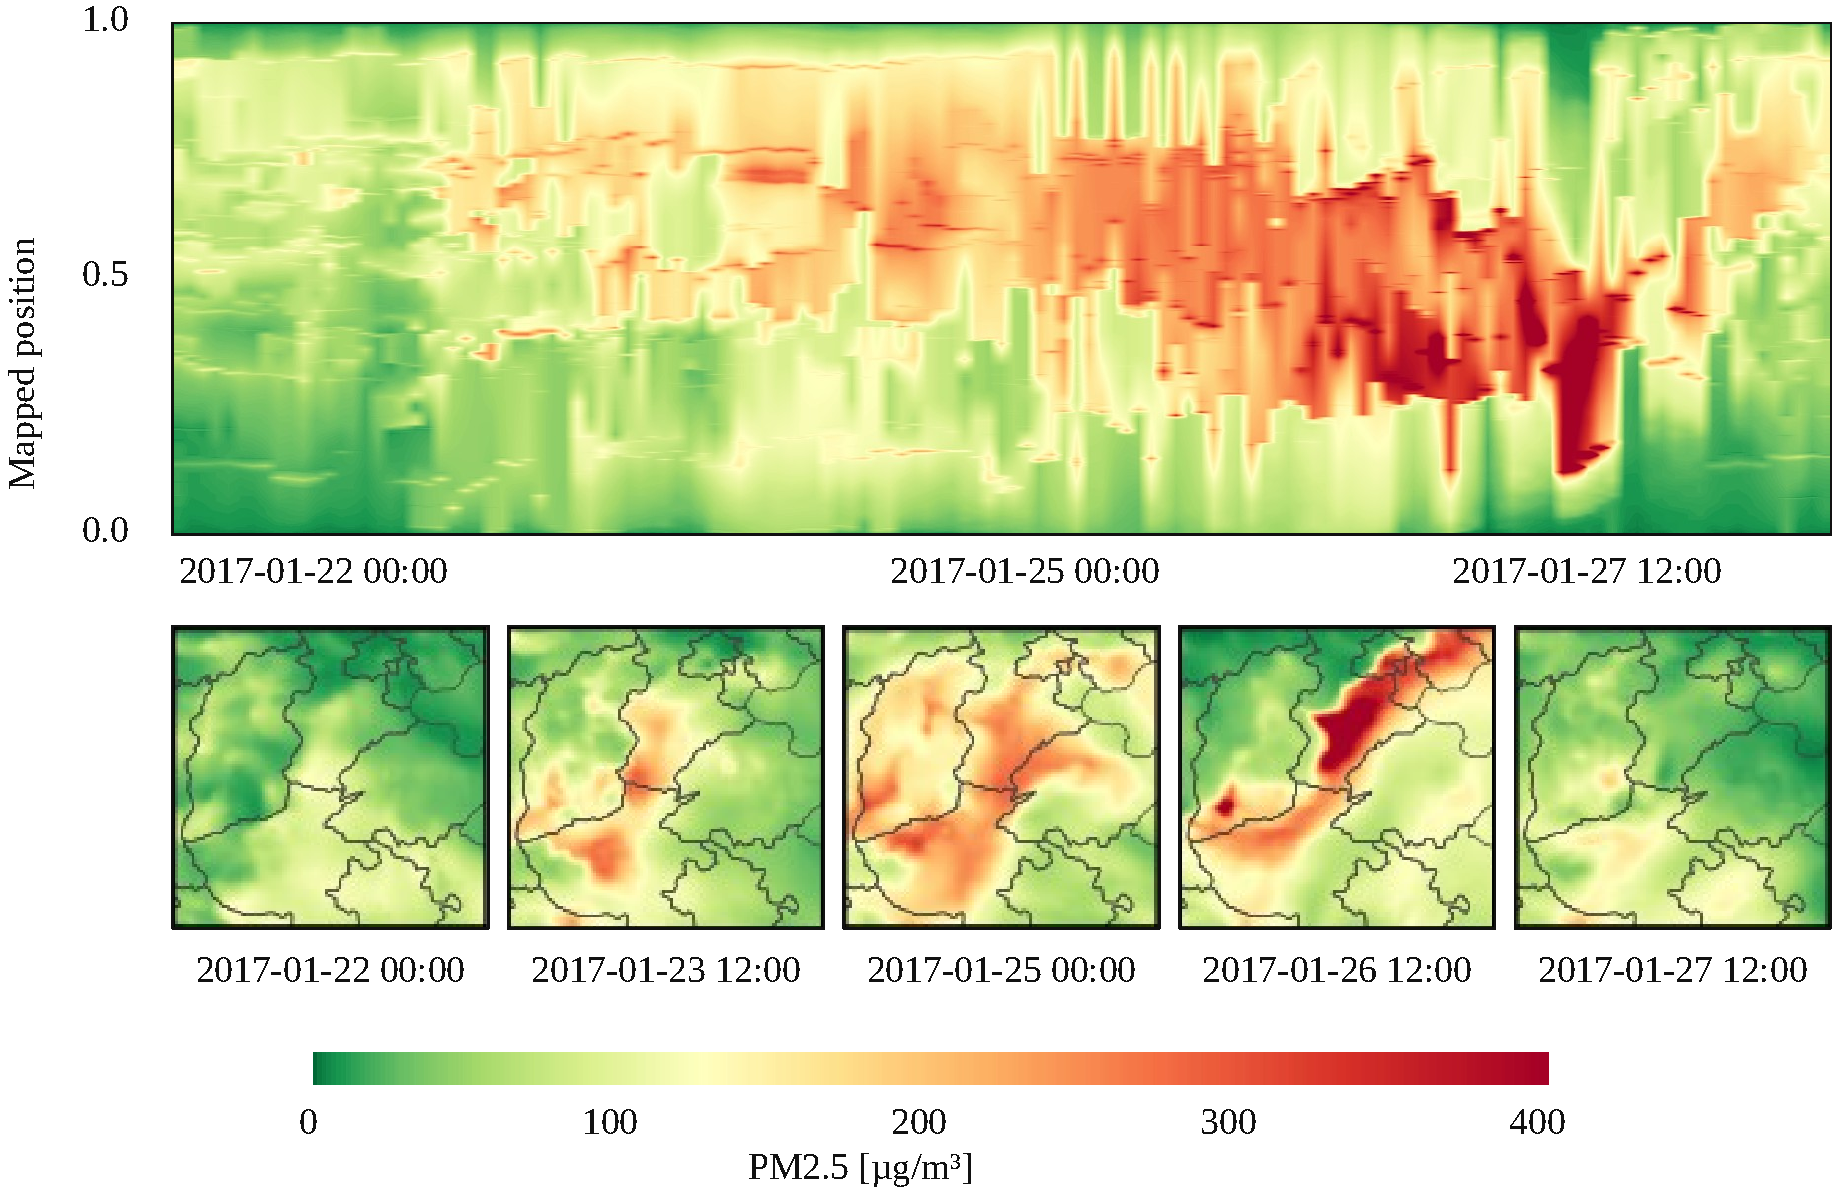
\includegraphics[width=\columnwidth]{figures/PM25_single_column.pdf}
\caption{Hourly PM2.5, January 22 00:00--27 12:00, 2017 (Beijing time): the 5\% map and five source snapshots. All 133 hourly samples are retained; concentrations above 400 $\mu$g/m$^3$ saturate.}
\label{fig:pm25-hourly}
\end{figure}
\paragraph{PM2.5.} Figure~\ref{fig:pm25-hourly} places a 133-hour event within the complete January sequence. Join trees of negated concentration represent high-concentration features, and the display restores positive concentration. The 5\% mode attains 4.998\% maximum merge error across all 744 hours. Snapshots provide the geographic context for the matched peak visible in the temporal map.

\subsection{Implementation and Runtime}
\paragraph{Verification pipeline.} The supplied code rebuilds the controlled-tree, feature-position and budget-distribution figures from labelled layouts and raster columns: 43 controlled overlaps, 364 controlled budgets, 9,168 planar frame--budget observations and 1,515 volumetric columns. For each volume column it reconstructs adjacent barriers from the original scalar raster, accumulates pairwise maxima and compares the complete fixed-label matrix with the source tree. It also verifies support IDs, interval order, canvas capacity, gaps and anchor slack. Every chart mark is then generated from the resulting CSV records. The five-sequence audit separately recomputes the point/width certificates and the baseline inversion errors in Table~\ref{tab:real-bounds}. These two checks link the rendered spatial-error distributions to the theoretical quantities used during ordering. Planar optimization takes 0.15--3.32\,s on the four benchmark inputs and 199.97\,s for the uncached PM2.5 Balanced run on Apple M4; full pipeline times and configurations appear in the supplement.

\paragraph{Configuration and runtime.} Tables~\ref{tab:anchor-parameters-final} and~\ref{tab:volume-parameters} give the fixed settings used by the quantitative comparisons. Only the merge allowance changes between each Exact--Balanced pair. The table runtimes measure one uncached run on Apple M4; optimization includes order search and anchor placement, while the total includes tree extraction, matching, filling and checks.
\begin{table}[!tb]
\centering
\caption{Planar parameter settings and runtime (seconds).}
\label{tab:anchor-parameters-final}
\footnotesize
\setlength{\tabcolsep}{2pt}
\renewcommand{\arraystretch}{0.95}
\begin{tabular}{@{}lccccc@{}}
\toprule
Parameter & Gaussian & Ring & Wildfires & Storms & PM2.5 \\
\midrule
$\varepsilon$ & 1\% & 1\% & 5\% & 10\% & 5\% \\
$N_r$ & 4096 & 196 & 4096 & 4096 & 4096 \\
$s_w$ & 0.00581 & 0.00328 & 0.00053 & 0.01170 & 0.00073 \\
$t_{opt}$ & 0.156 & 0.150 & 3.324 & 2.600 & 199.975 \\
$t_{total}$ & 1.340 & 0.486 & 4.424 & 63.447 & 231.177 \\
\bottomrule
\end{tabular}
\vspace{2pt}
\begin{minipage}{0.94\columnwidth}\footnotesize Weights $(4,1,0.5,0.1)$ and $\rho=0.5$ are fixed. $s_w$ is width per support measure; $N_r$ is raster length. PM2.5 uses $p=5\%$ of per-frame range and a fixed 5\% Balanced budget, without validation-set selection; both times are remeasured without a tree cache under the same pipeline scope. Times are one run on Apple M4: optimization and full pipeline, respectively.\end{minipage}
\end{table}

\begin{table}[!tb]
\centering
\caption{Volumetric datasets and Balanced-mode parameter settings.}
\label{tab:volume-parameters}
\footnotesize
\setlength{\tabcolsep}{2pt}
\renewcommand{\arraystretch}{0.95}
\begin{tabular}{@{}lcc@{}}
\toprule
Parameter & Cylinder & Tangaroa \\
\midrule
Frames & 102 & 201 \\
Grid & $135\times64\times48$ & $300\times180\times120$ \\
Scalar & $Q$-criterion & Speed $\|\mathbf{v}\|$ \\
Persistence & 2\% per-frame range & 0.2 absolute \\
Reference & $+x$ & $+x$ \\
$\varepsilon$ & 1\% & 33.33\% \\
$N_r$ & 32768 & 131072 \\
$s_w$ & $2.70668\times10^{-5}$ & 0.40953 \\
Weights & $(0.1,16,0,0.1)$ & $(0,64,0,0)$ \\
$\rho$ & 1 & 1 \\
Gap$/L_{world}$ & $1/300$ & $1/960$ \\
Extra$/L_{world}$ & 0.1 & 0.1 \\
\bottomrule
\end{tabular}
\vspace{2pt}
\begin{minipage}{0.94\columnwidth}\footnotesize Weights are reference, geometry, temporal and eccentricity. $s_w$ is width per support measure (Cylinder voxel counts; Tangaroa physical volume); $N_r$ is raster length, distinct from the physical canvas extent $L_{world}$. Exact uses zero allowance with the same other parameters as its Balanced counterpart.\end{minipage}
\end{table}

\Needspace{7\baselineskip}

\section{Discussion and Conclusion}\label{sec:discussion}
Keeping merge-tree topology has an unavoidable positional cost. The point bound isolates the part forced by subtree ordering; the width-aware and bounded-error results identify restrictions that remain when intervals and a merge allowance are included. AnchorMTM follows this analysis by selecting an order before optimizing its placement. The evidence connects controlled optima to temporal feature trajectories: relaxation acts on a difficult tail in Storms and on most frames in the two default volume configurations.

The fixed coordinate supports location and motion along the chosen direction, while relative geometry and hierarchical unfolding support different readings. Neighborhood preservation is therefore a separate objective, as the curve comparisons and Cylinder guidance case illustrate. A single projection merges differences perpendicular to that direction, and matching quality affects the motion samples used to estimate it. Source snapshots and analyst-selected directions provide complementary context. Finite-width ordering remains heuristic; a residual certificate gap may reflect the search or a non-tight bound. The distinct objectives of the case configurations make these choices explicit and motivate tighter ordering methods and task-based evaluation of the anchored coordinate.

AnchorMTM thus provides a temporal merge tree map whose positions are read against one fixed spatial reference. The bounds quantify the hierarchical restrictions, the merge budget controls which constraints may be released, and checked reconstruction carries that choice into the displayed map.

\FloatBarrier
\begingroup
\interlinepenalty=10000
\bibliographystyle{abbrv-doi-narrow}
\bibliography{references}
\endgroup
\end{document}
